% Digital adiabatic: prep + one Trotter layer of H(s), then measure at the end
% سبک مشترک نمودارهای سند پایه‌ها (فقط داخل محیط latin فراخوانی شود)
\tikzset{
	qafbox/.style={
		draw=black!55,
		rounded corners=2pt,
		align=center,
		inner sep=3pt,
		thick,
		fill=white,
		font=\footnotesize\linespread{1}\selectfont,
		minimum height=0.95cm
	},
	qafwide/.style={
		qafbox,
		text width=2.55cm
	},
	qafnarr/.style={
		qafbox,
		text width=2.05cm
	},
	qaftitle/.style={
		font=\small\bfseries\linespread{1}\selectfont,
		align=center
	},
	qafarr/.style={
		-{Latex[length=2.2mm]},
		thick,
		draw=black!65
	},
	qafpanel/.style={
		draw,
		thick,
		rounded corners=4pt,
		inner xsep=8pt,
		inner ysep=8pt
	}
}

\begin{tikzpicture}[
	x=0.82cm,
	y=0.95cm,
	font=\footnotesize,
	note/.style={font=\scriptsize, text=black!55}
	]
	\draw[thick] (0,2) -- (10.8,2);
	\draw[thick] (0,0.6) -- (10.8,0.6);
	\node[left] at (0,2) {$q_0$};
	\node[left] at (0,0.6) {$q_1$};

	\node[qafbox, fill=blue!12, minimum width=0.65cm, minimum height=0.5cm] at (0.85,2) {$H$};
	\node[qafbox, fill=blue!12, minimum width=0.65cm, minimum height=0.5cm] at (0.85,0.6) {$H$};
	\node[note] at (0.85,2.55) {$\lvert++\rangle$};

	\draw[thick, densely dashed] (1.55,-0.05) rectangle (8.55,2.7);
	\node[note] at (5.05,3.0) {layer $k$: $s_k=(k+\tfrac12)/N$,\; $\Delta t=T/N$};

	\node[qafbox, fill=orange!14, minimum width=1.2cm, minimum height=0.5cm] at (2.55,2) {$R_x(-2a)$};
	\node[qafbox, fill=orange!14, minimum width=1.2cm, minimum height=0.5cm] at (2.55,0.6) {$R_x(-2a)$};

	\fill (4.2,2) circle (2.1pt);
	\fill (4.2,0.6) circle (2.1pt);
	\draw[thick] (4.2,2) -- (4.2,0.6);
	\node[qafbox, fill=green!12, minimum width=1.4cm, minimum height=0.48cm] at (5.35,1.3) {$R_{zz}(-2b)$};

	\node[qafbox, fill=cyan!12, minimum width=1.2cm, minimum height=0.5cm] at (7.15,2) {$R_z(-2c)$};
	\node[qafbox, fill=cyan!12, minimum width=1.2cm, minimum height=0.5cm] at (7.15,0.6) {$R_z(-2c)$};

	\node[qafbox, fill=gray!14, minimum width=0.8cm, minimum height=0.5cm] at (9.7,2) {$Z$};
	\node[qafbox, fill=gray!14, minimum width=0.8cm, minimum height=0.5cm] at (9.7,0.6) {$Z$};
	\node[note] at (9.7,2.55) {readout};

	\node[note, align=left] at (5.2,-0.75) {%
		$a=(1-s)h_x\Delta t$,\quad $b=sJ\Delta t$,\quad $c=sh_z\Delta t$};
\end{tikzpicture}
